\documentclass{article}
\usepackage[utf8]{inputenc}

\title{Interrupciones}
\author{Christofer Fabián Chávez Carazas}
\date{September 2016}

\usepackage{natbib}
\usepackage{graphicx}
\usepackage{float}


\begin{document}

\maketitle

\section{Acceso}

\subsection{Windows}

\begin{enumerate}
    \item Teclear 'msinfo32' en Ejecutar.
    \item Entrar en 'Recursos de hardware'
    \item Entrar en 'IRQs' 
\end{enumerate}

La lista de todos los IRQs asignados al sistema aparecerán allí.

\begin{figure}[h]
\centering
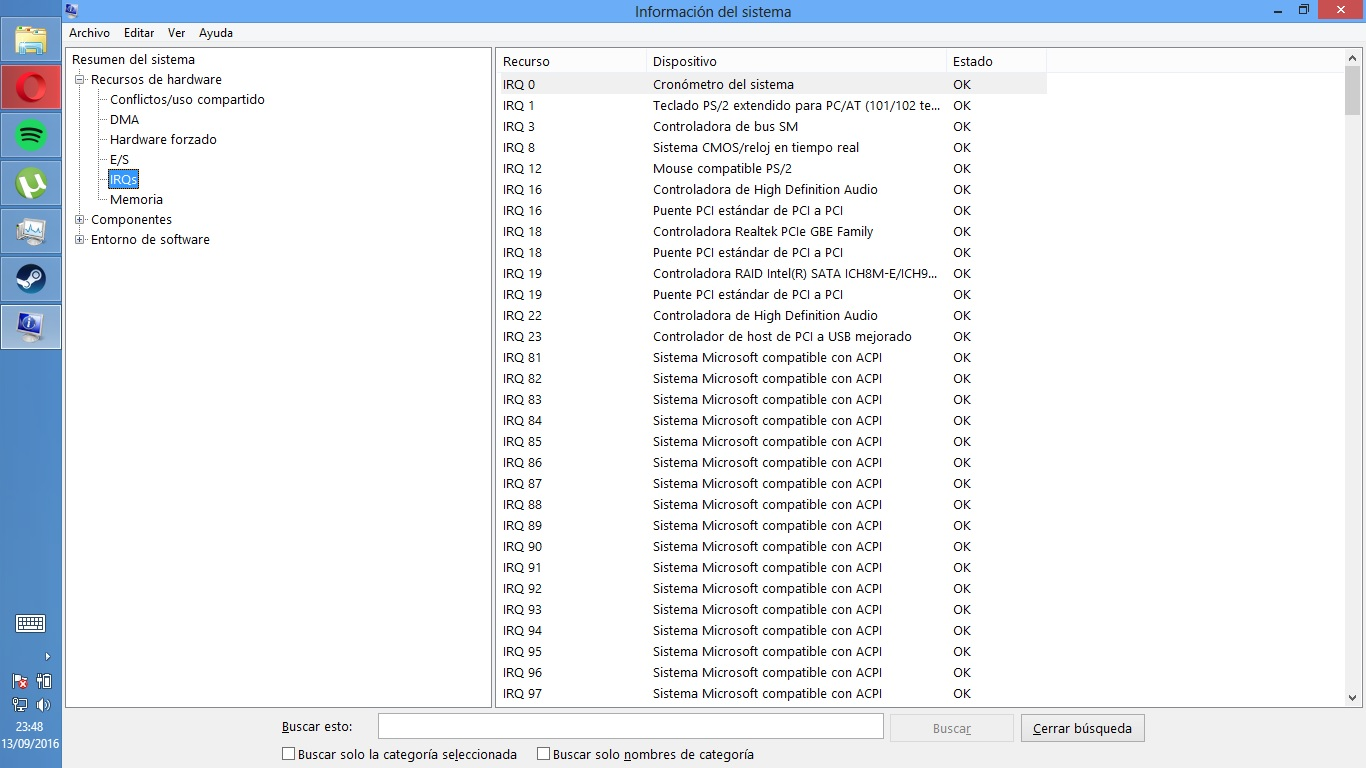
\includegraphics[scale=0.35]{windows.jpg}
\label{Lista de IRQs en Windows}
\caption{Lista de IRQs en Windows}
\end{figure}

\section{Linux}

Abrimos una terminal y tecleamos el siguiente comando: \textbf{\$ cat /proc/interrupts}.

\begin{figure}[h]
\centering
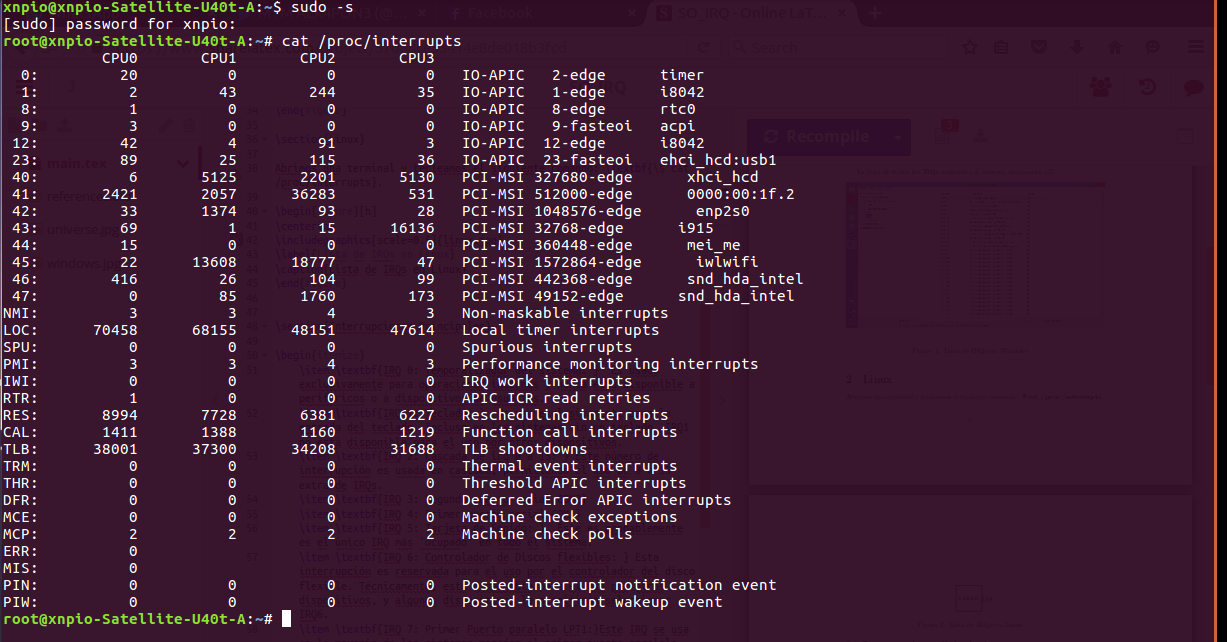
\includegraphics[scale=0.3]{linux.png}
\label{Lista de IRQs en Linux}
\caption{Lista de IRQs en Linux}
\end{figure}


\section{Interrupciones Principales}

\begin{itemize}
    \item \textbf{IRQ 0: Temporalizador del sistema: }  Es usado exclusivamente para operaciones internas y nunca esta disponible a periféricos o a dispositivos de usuarios.
    \item \textbf{IRQ 1: Teclado: }  Se usa exclusivamente para la entrada del teclado. Incluso en los sistemas sin un teclado, IRQ1 no está disponible para el uso por otros dispositivos.
    \item \textbf{IRQ 2: Cascada de irq 8 a 15: } Este número de interrupción es usada en cascada, permitiendo el uso de 8 a 15 extra de IRQs.
    \item \textbf{IRQ 3: Segundo puerto serial COM2}
    \item \textbf{IRQ 4: Primer puerto serial COM1}
    \item \textbf{IRQ 5: Tarjeta de Sonido: }  Éste es probablemente es el único IRQ más 'ocupado' en todo el sistema.
    \item \textbf{IRQ 6: Controlador de Discos flexibles: } Esta interrupción es reservada para el uso por el controlador del disco flexible. Técnicamente, está disponible para el uso por otros dispositivos, y algunos dispositivos le permitirán seleccionar IRQ6.
    \item \textbf{IRQ 7: Primer Puerto paralelo LPT1:}Este IRQ se usa en la mayoría de los sistemas manejar el primer puerto paralelo, normalmente para el uso de una impresora.
    \item \textbf{IRQ 8: Sistema reloj en tiempo real:} Este cronómetro se usa por los programas del software para manejar eventos que deben calibrarse a tiempo del real-mundo; esto se hace poniendo alarmas que activan esta interrupción en un momento especificado.
    \item \textbf{IRQ 9,10,11: }  Interrupciones disponibles para periféricos extra.
    \item \textbf{IRQ 12: PS/2 mouse: }  En máquinas que usan un ratón de PS/2, esto está que el IRQ reserva para su uso. Usando un ratón de PS/2 libera al puerto serial COM1 y la interrupción usa (IRQ4) para otros dispositivos.
    \item \textbf{IRQ 13: Coprocesador matemático, operaciones de punto flotante: } Es la interrupción reservada para la unidad del punto flotante integrada en el coprocesador de la matemática. Se usa exclusivamente para la señalización interna y nunca está disponible para el uso por periféricos.
    \item \textbf{IRQ 14: Primary IDE channel: } En la mayoría de computadoras este IRQ es reservado para el uso por el controlador de IDE primario que proporciona el acceso a los primeros dos dispositivos de IDE/ATA (normalmente el disco duro maneja y/o CD-ROM maneja).
    \item \textbf{IRQ 15: Secondary IDE channel: } Es complementario al IRQ 14.
\end{itemize}


%\bibliographystyle{plain}
%\bibliography{references}
\end{document}
